\section{Ueber den Veranstalter und unsere Cryptoparty}
  \begin{frame}{Das FIfF}
    Forum InformatikerInnen für Frieden und gesellschaftliche Verantwortung e.V.
  \end{frame}
  \begin{frame}{Das Medienzentrum}
    MZM - Medienzentrum München des\\
    JFF -- Institut für Medienpädagogik in Forschung und Praxis\\
    JFF -- Jugend Film Fernsehen e.V.
  \end{frame}
  \begin{frame}{Der Chaos Computer Club - Was tun wir?}
    \begin{itemize}
      \item{Kreativer Umgang mit Technik...}
      \item{... und deren Auswirkungen auf die Gesellschaft}
      \item{soll sagen: Auf Chancen hinweisen, vor Risiken warnen}
      \item{Viele Leute (\textasciitilde 130 Mitglieder), viele Themen}
      \item{Kunst, Kultur und Wissenschaft fördern}
      \item{Immer: Spaß am Gerät}
    \end{itemize}
  \end{frame}
  \begin{frame}{Der Chaos Computer Club - Wer sind wir?}
    \begin{itemize}
      \item{Eine galaktische Gemeinschaft von Lebewesen,}
      \item{unabhängig von Alter,}
      \item{Geschlecht,}
      \item{Rasse}
      \item{sowie gesellschaftlicher Stellung}
    \end{itemize}
  \end{frame}
  \begin{frame}{Die Cryptoparty}
    \begin{itemize}
      \item{Wir zeigen euch wie ihr Verschlüsselungstechniken für euch nutzen könnt}
      \begin{itemize}
        \item{Passwort-Management}
        \item{Anonyme(re)s Web-Surfen}
        \item{E-Mail-Verschlüsselung und -Signatur}
        \item{\ldots und mehr auf Anfrage}
      \end{itemize}
    \end{itemize}
  \end{frame}
  %\begin{frame}{Internetzugang}
  %  \begin{itemize}
  %    \item{lrz}
  %    \item{eduroam}
  %  \end{itemize}
  %\end{frame}

\section{``Theorie'' oder Einführende Worte}
  \begin{frame}{Warnhinweise}
    \begin{itemize}
      \item 100 \%-ige Sicherheit gibt es nicht
      \item Ziel von Absicherung ist es
      \begin{itemize}
        \item Angriffe \textit{teurer} zu machen
        \item und \textit{nicht}, sie unmöglich zu machen
      \end{itemize}
      \item vor gezielten Angriffen, hinter denen viele Ressourcen (Geld) stecken, kann man sich kaum schützen
    \end{itemize}
  \end{frame}
  \begin{frame}{Wichtige Fragen für Euch}
    \begin{itemize}
      \item \textbf{Was} soll geschützt werden?
        \begin{itemize}
          \item Anonymität
          \item Echtheit des Gegenübers (Authentizität)
          \item Vertraulichkeit der Daten
          \item \ldots
        \end{itemize}
      \item \textbf{Wem vertraut} Ihr?
    \end{itemize}
  \end{frame}

  \begin{frame}{Vertrauen}
    \textbf{Woher weiß man, wem oder was man vertrauen kann?}
    \begin{itemize}
      \item Kurze Antwort: weiß man \textbf{nicht}.
      \item Lange Antwort
      \begin{itemize}
        \item es gibt Fragen, die man stellen kann\ldots
        \item {\ldots}und es gibt das Bauchgefühl.
      \end{itemize}
    \end{itemize}
  \end{frame}
\begin{frame}{Welche Fragen kann man stellen?}
  \begin{itemize}
    \item \textbf{Wo} sind meine Daten?
    \begin{itemize}
      \item Auf einem Blatt Papier zuhause in meiner Schublade.
      \item Auf meinem Computer: Wie gut ist die Software \textbf{überprüfbar}, die meine Daten verwaltet?
        \begin{itemize}
          \item Open Source (in menschenlesbarer Form öffentlich):\\gut überprüfbar
          \item Closed Source (nur in maschinenlesbarer Form öffentlich):\\nicht überprüfbar
        \end{itemize}
      \item In der Cloud: \textbf{Wer} betreibt einen Dienst\\und \textbf{welche Motivation} hat der Betreiber?
        \begin{itemize}
          \item Macht der Betreiber einen vertrauenswürdigen Eindruck?
          \item Womit verdient der Betreiber sein Geld?
          \item Inwieweit ist man bereit,\\ \textbf{Komfort gegen Kontrolle einzutauschen}?
        \end{itemize}
    \end{itemize}
  \end{itemize}
\end{frame}

  \begin{frame}{Meta- und Nutzdaten}
    \begin{itemize}
      \item Meta-/Verbindungsdaten
      \begin{itemize}
        \item E-Mail: Wer hat wann an wen mit welcher Betreffzeile eine E-Mail geschickt?
        \item Surfen: Wer hat wann welche Webseite besucht?
        \item Mobilfunk: Wer hat wann von wo mit wem kommuniziert?
      \end{itemize}
      \item Nutz-/Inhaltsdaten
      \begin{itemize}
        \item E-Mail: Was waren Inhalt und Anhänge?
        \item Surfen: Welche Inhalte waren auf der Webseite?
        \item Mobilfunk: Was wurde geschrieben oder gesprochen?
      \end{itemize}
    \end{itemize}
  \end{frame}

  \begin{frame}{Kryptographie auf einer Folie}
    \begin{itemize}
      \item Symmetrisch: \textit{ein} \textbf{geheimer} ``Schlüssel'' (= lange Zahl)
      \begin{itemize}
        \item braucht einen \textbf{vertraulichen Kanal} zur Vereinbarung eines Schlüssels zwischen zwei Kommunikationspartnern
        \item Anwendungsfälle
        \begin{itemize}
          \item Festplattenverschlüsselung
          \item Zip-Dateien mit Passwort
        \end{itemize}
      \end{itemize}
      \item Asymmetrisch: ein \textbf{geheimer} \textit{und} ein dazu passender \textbf{öffentlicher} Schlüssel bilden ein \textbf{Schlüsselpaar}
      \begin{itemize}
        \item braucht einen \textbf{authentischen}, aber \textit{keinen vertraulichen} Kanal zur sicheren Zuordnung des Schlüssels zu einer Person
        \item Verwendung
          \begin{itemize}
            \item Verschlüsseln mit öffentlichem Schlüssel,\\Entschlüsseln mit geheimem Schlüssel
            \item \textit{Digitale Signatur} von Daten mit dem privaten Schlüssel\\als Echtheitsbestätigung
          \end{itemize}
      \end{itemize}
    \end{itemize}
  \end{frame}

\section{Passwörter}
  \begin{frame}{Passwörter}
    \Large Wer hat mindestens fünf Online-Accounts? 
  \end{frame}
  \begin{frame}{Passwörter}
    \Large Und wer hat dafür mindestens drei verschiedene Passwörter?
  \end{frame}
  \begin{frame}{Sichere Passwörter?}
    \begin{itemize}
      \item Ideal: Jedes Passwort nur einmal verwenden\\
      \small Besonders wichtig bei E-Mail-Accounts, da ``Passwort zurücksetzen''-Funktionen oft per E-Mail funktionieren \normalsize
      \item Besser als überall das gleiche Passwort:\\Passwörter leicht variieren (``salzen'')
      \begin{itemize}
        \item 1Quastenfl0sser.mai für Mail
        \item 1Quastenfl0sser.son für Social Network
        \item \ldots
      \end{itemize}
      \item Oder: Passwort-Manager
    \end{itemize}
  \end{frame}
  \begin{frame}{Passwort-Manager}
    \begin{itemize}
      \item Software zur Verwaltung von Passwörtern
      \item Datenbank wird mit einem Master-Passwort verschlüsselt
      \item Beispiel: KeePassX (Open Source)
    \end{itemize}
      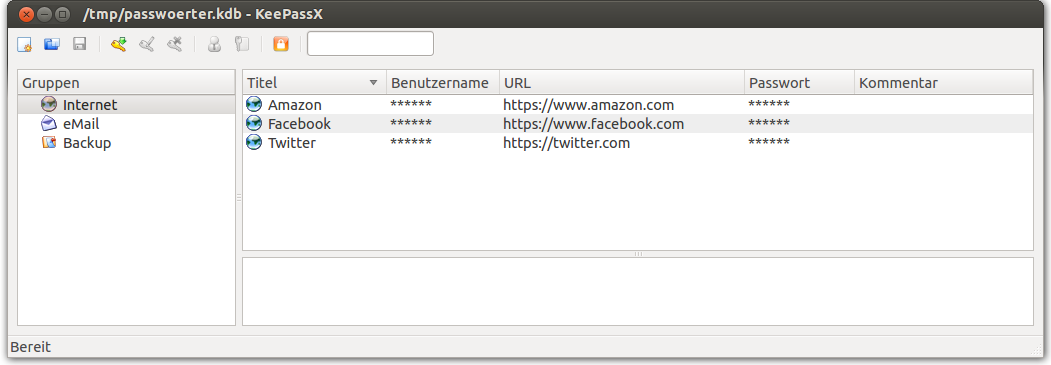
\includegraphics[width=\textwidth]{images/keepassx.png}
    \begin{itemize}
      \item \textbf{Wichtige Passwörter trotzdem merken!}
      \item \ldots oder zumindest auf einem Zettel aufschreiben und zuhause an einem sicheren Ort lagern
    \end{itemize}
  \end{frame}
  \begin{frame}{Aber wie soll man sich Passwörter merken?}
    \begin{center}
      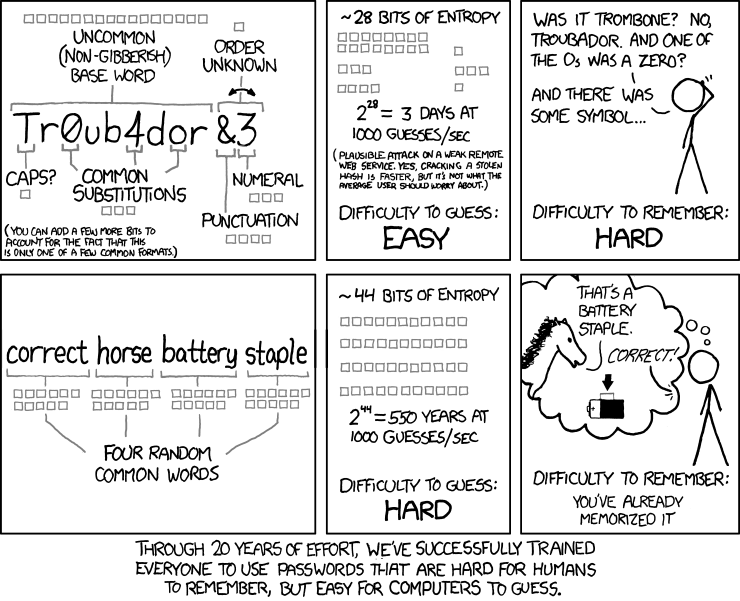
\includegraphics[width=0.9\textheight]{images/password_strength.png}\\
    \end{center}
    \tiny Quelle: \url{http://xkcd.com/936/}
  \end{frame}
\section{Web-Surfen}
  \begin{frame}{Anonymes Werbsurfen}
    \begin{itemize}
      \item Anfallende Meta-Daten
      \begin{itemize}
        \item Cookies und Co (HTML5 Persistent Local Storage, Flashcookies, \ldots)
        \item Browser-Fingerabdruck
        \item IP-Adresse
      \end{itemize}
      \item Wie kann man trotzdem anonym\textit{er} surfen?
      \begin{itemize}
        \item \textbf{Einfach}: Tor Browser Bundle (Open Source)\\ \url{https://www.torproject.org}\\[.5cm]
        \item \textbf{Ohne Spuren am PC}: Tails (Open Source)\\ \url{https://tails.boum.org}\\[.5cm]
        \item Alternative: Browser-Plugins
          \begin{itemize}
            \item NoScript, ClickToPlugin, AdBlockPlus, Ghostery (Achtung: Closed Source), \ldots 
          \end{itemize}
      \end{itemize}
    \end{itemize}
  \end{frame}

\section{E-Mail}
  \begin{frame}{E-Mails: Was soll geschützt werden?}
    E-Mails können
    \begin{itemize}
      \item abgehört
      \item gefälscht
    \end{itemize}
    werden. Deshalb stellen wir vor, wie man
    \begin{itemize}
      \item die Vertraulichkeit (das ``Briefgeheimnis'') umsetzt
      \\ $\Rightarrow$ Verschlüsselung
      \item die Echtheit des Gegenübers sicherstellt
      \\ $\Rightarrow$ Digitale Signatur
    \end{itemize}
  \end{frame}

  \begin{frame}{Analogie zur Vertraulichkeit von E-Mails}
    \begin{itemize}
      \item E-Mails sind ``Postkarten''
      \item diese werden in ``gläsernen Fahrzeugen'' transportiert
      \begin{itemize}
        \item ``Autobahnbetreiber'' kann alles mithören
        \item ``Post'' kann alles mithören
      \end{itemize}
      \item Bei \textbf{Transportverschlüsselung} ersetzt die ``Post'' die ``gläsernen Fahrzeuge'' durch ``undurchsichtige Fahrzeuge''
      \begin{itemize}
        \item ``Autobahnbetreiber'' kann mithören,\\welche ``Post'' mit welcher anderen ``Post'' kommuniziert
        \item ``Post'' kann alles mithören
      \end{itemize}
      \item Bei \textbf{Ende-zu-Ende-Verschlüsselung} steckt der Absender die ``Postkarte'' in einen ``Briefumschlag''
      \begin{itemize}
        \item ``Autobahnbetreiber'' kann mithören,\\wer mit wem kommuniziert
        \item ``Post'' kann mithören, wer mit wem kommuniziert
      \end{itemize}
      \item Wir stellen hier Ende-zu-Ende-Verschlüsselung vor.
    \end{itemize}
  \end{frame}

  \begin{frame}{Überprüfung der Echtheit}
  Was muss A tun, er an B eine Nachricht schicken will, aber nicht seinen öffentlichen Schlüssel kennt?\\
  \begin{enumerate}
    \item Im ``Telefonbuch'' nach dem Schlüssel suchen
    \item Echtheit mit Hilfe eines \textbf{vertrauenswürdigen Dritten} C\\überprüfen
  \end{enumerate}
  \begin{center}
    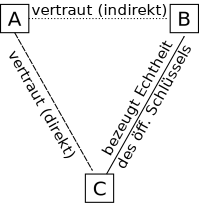
\includegraphics[width=0.5\textheight]{images/vertrauen.pdf}
  \end{center}
  \end{frame}

  \begin{frame}{Wie stellt man Vertrauen her?}
    \begin{itemize}
      \item S/MIME -- Hierarchischer Vertrauensansatz
      \begin{itemize}
        \item Es gibt ``zentrale Vertrauensinstanzen'' (Certification Authorities, CAs), denen \textbf{jeder} vertraut
        \item Diese bestätigen die Echtheit der Schlüssel von  \textit{untergeordneten} CAs
        \item \ldots eine (beliebige) CA aus der Vertrauenskette kann die Echtheit von Schlüsseln von Personen bestätigen
        \item wird hier \textit{nicht} behandelt
      \end{itemize}
      \item GnuPG -- Dezentraler Vertrauensansatz
      \begin{itemize}
        \item jeder kann festlegen, wem er vertraut
        \begin{itemize}
          \item er kann die Echtheit eines Schlüssels z.B. bei einem persönlichen Treffen überprüfen
        \end{itemize}
        \item jeder \textit{kann} sein Vertrauensnetz veröffentlichen (Web-of-Trust)
        \begin{itemize}
          \item Vorteil: Man kann auch ``Freunden von Freunden'' vertrauen
          \item Nachteil: Beziehungen zwischen Menschen sind öffentlich 
        \end{itemize}
        \item wird hier behandelt
      \end{itemize}
    \end{itemize}
  \end{frame}

  \begin{frame}{E-Mail-Absicherung mit GnuPG}
    \begin{centering}
      \Huge Live-Demo
    \end{centering}
  \end{frame}

\section{Fragen, Feedback}
  \begin{frame}{Fragen, Feedback, ...}
    \begin{itemize}
      \item{Her damit!}
      \item{Fragen an alle Helfer (bitte gebt Euch zu erkennen :-)}
      \item{Link: \url{https://muc.pads.ccc.de/cryptoparty}}
    \end{itemize}
  \end{frame}
